%-------------------------------------------------------------------------------
% jack
%-------------------------------------------------------------------------------
%
% \file        jack.tex
% \library     Documents
% \author      Chris Ahlstrom
% \date        2016-01-28
% \update      2021-02-07
% \version     $Revision$
% \license     $XPC_GPL_LICENSE$
%
%     Provides the JACK page section of seq24-user-manual.tex.
%
%-------------------------------------------------------------------------------

\section{Seq66 JACK Support}
\label{sec:jack}

   This section describes some details concerning the JACK support of
   \textsl{Seq66}.
   As with \textsl{Seq24}, \textsl{Seq66} has JACK transport support.
   JACK supposedl works with \textsl{Windows}, but we do not provide a JACK
   MIDI engine for that system.
   The JACK support is loosely based on the RtMIDI project
   (see \cite{rtmidi}).
   This mode also supports fallback-to-ALSA if the JACK
   server is not running.

   If one wants to use \textsl{Seq66} and USB devices
   with JACK MIDI, one needs to expose the USB ports to JACK using
   \texttt{a2jmidid -{}-export-hw}, and connect the resultant MIDI JACK ports
   oneself, using \textsl{QJackCtl}, for example.

   To enable the JACK transport support at run-time on
   \textsl{Linux}, the options
   \texttt{-j}/\texttt{-{}-jack-transport},
   \texttt{-J}/\texttt{-{}-jack-master},
   \texttt{-C}/\texttt{-{}-jack-master-cond},
   and \texttt{-t}/\texttt{-{}-jack-midi} are available.

   The following sections discuss the JACK transport support and the native
   JACK MIDI support.

\subsection{Seq66 JACK Transport}
\label{subsec:jack_transport}

   JACK transport support is \textsl{separate} from native JACK MIDI support.
   The JACK transport client is an invisible client with the
   name "seq66-transport", while the JACK MIDI client is visible in
   \textsl{QJackCtl}, and the ports created are part of the
   "seq66" client.

%  TRUE? :
%  The first thing to note about JACK transport with \textsl{Seq66} is
%  that the progress bars will not move unless \textsl{Seq66} is
%  connected to a JACK client, such as \textsl{Hydrogen} (in JACK MIDI mode)
%  or \textsl{Yoshimi}.

   \textsl{Seq66} can be configure to run without JACK transport, with JACK
   transport as a "slave" (i.e. "client"), as JACK master, or as JACK master if
   there is no other master detected.

   As per the rules of JACK, any client can start and stop the transport, and
   the other clients will follow suit.  When \textsl{Seq66} is a JACK client,
   it will accept beats/minute (BPM) changes from another client that is
   running as master.  When \textsl{Seq66} is master, changes to its BPM will
   be transmitted to the other clients.

\subsection{Seq66 Native JACK MIDI}
\label{subsec:jack_native_midi}

   Currently, \textsl{Seq66} will connect to a JACK
   client automatically only at startup, where it will connect to all JACK
   clients that it finds.  If it can't find a JACK client, then it will
   fail to register a JACK port, and cannot play.

   The other option is to set up virtual ports using the
   \texttt{-{}-manual-ports} or \texttt{-{}-options virtual=o,i} options, and then
   to manually connected these ports to the desired MIDI devices or
   applications using \textsl{QJackCtl} (for example).

   To run with JACK MIDI, just make sure JACK is running, then start
   \textsl{Seq66}, which will detect JACK and use it.
   If it instead opts to run with ALSA, edit the 'rc' file to set up
   \texttt{midi\_jack}, or add the
   \texttt{-t} or \texttt{-{}-jack-midi}
   option to the command-line.
   If \textsl{Seq66} doesn't find JACK, it will still fall back to ALSA.

	\index{sticky options}
   The JACK (\texttt{-t}) and ALSA (\texttt{-A}) options are sticky options.
   That is, they are saved to the 'rc' configuration file at exit,
   so one does not have to specify them in subsequent \textsl{seq66} sessions.

\subsubsection{Seq66 JACK MIDI Output}
\label{subsubsec:jack_midi_output}

   By default (or depending on the 'rc' configuration file),
   \textsl{Seq66} will
   \index{jack!auto-connect}
   \index{auto-connect}
   automatically connect the ports that it finds to \texttt{seq66}.
   The following figure shows connections to a number of USB MIDI devices
   (purple) that have been bridged to JACK (red) by the \texttt{a2jmidid}
   daemon.

\begin{figure}[H]
   \centering 
   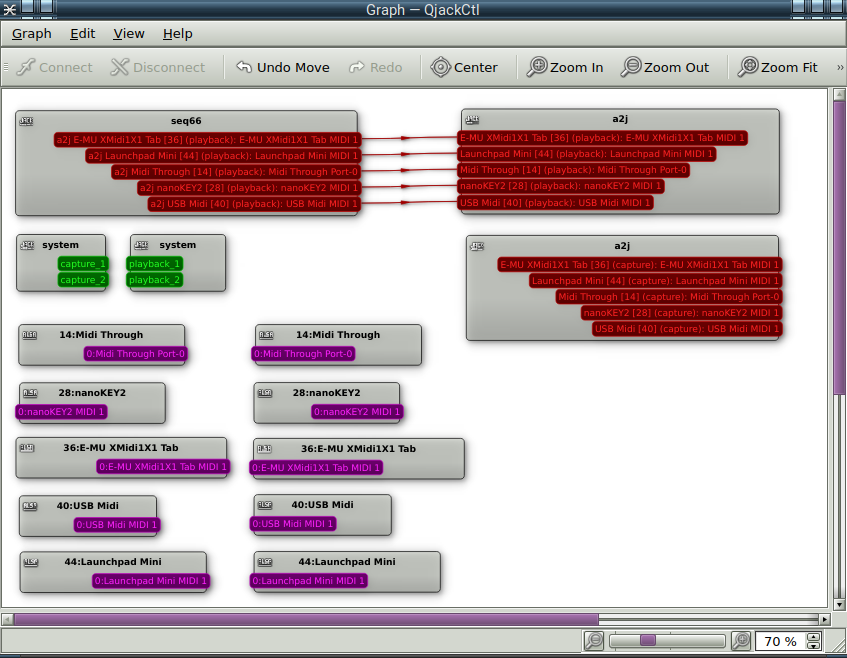
\includegraphics[scale=0.40]{jack/qjackctl-a2j-graph.png}
   \caption{JACK MIDI Ports and Auto-Connect}
   \label{fig:jack_midi_ports_auto_connect}
\end{figure}

   Note that the ports in \textsl{Seq66} are named after the devices to which
   they are connected.

	The output ports available are shown in \textsl{seq66}'s
	\textbf{Edit / Preferences / MIDI Clock} tab.
   If USB devices are not shown, that means
   that the \texttt{a2jmidid} is not running.
   There is a \texttt{bash} script, \texttt{data/linux/startjack}
   that will run \texttt{jack\_control} and \texttt{a2j\_control} to start JACK
   and the "a2j" daemon to provide full support.
   On our current setup, it creates devices with long names (abbreviated inside
   \textsl{Seq66}):

   \begin{verbatim}
6    # number of MIDI clocks (output busses)
 0 0 "[0] 0:0 seq66:a2j Midi Through [14] (playback): Midi Through Port-0"
 1 0 "[1] 0:1 seq66:a2j Launchpad Mini [28] (playback): Launchpad Mini MIDI 1"
 2 0 "[2] 0:2 seq66:a2j E-MU XMidi1X1 Tab [32] (playback): E-MU ... Tab MIDI 1"
 3 0 "[3] 0:3 seq66:a2j nanoKEY2 [36] (playback): nanoKEY2 MIDI 1"
 4 0 "[4] 0:4 seq66:a2j USB Midi [40] (playback): USB Midi MIDI 1"
 5 0 "[5] 1:5 seq66:yoshimi-01 midi in"
   \end{verbatim}

\subsubsection{Seq66 JACK MIDI Input}
\label{subsubsec:jack_midi_input}

   The input ports also end up with long names:

   \begin{verbatim}
5   # number of input MIDI busses
0 1 "[0] 0:0 seq66:a2j Midi Through [14] (capture): Midi Through Port-0"
1 1 "[1] 0:1 seq66:a2j Launchpad Mini [28] (capture): Launchpad Mini MIDI 1"
2 1 "[2] 0:2 seq66:a2j E-MU XMidi1X1 Tab [32] (capture): E-MU ... Tab MIDI 1"
3 0 "[3] 0:3 a2j:nanoKEY2 [36] (capture): nanoKEY2 MIDI 1"
4 0 "[4] 0:4 a2j:USB Midi [40] (capture): USB Midi MIDI 1"
   \end{verbatim}

   When the check-box for a buss is selected, that input can be captured by
   \texttt{seq66}.

\subsubsection{Seq66 JACK MIDI Virtual Ports}
\label{subsubsec:jack_midi_virtual_ports}

   \index{ports!manual}
   \index{ports!virtual}
   The manual-versus-normal port support for JACK MIDI is essentially the same
   as that for ALSA.
   The \texttt{-{}-manual-ports} and
   \texttt{-{}-options virtual=o,i} options provide
   "virtual ports".  These are ports that do not represent
   hardware, but are created by applications to allow them to connect to other
   applications or MIDI devices.

   The difference between manual/virtual ports and normal ports is that, while
   normal ports are automatically connected to the remote ports that exist in
   the system, the manual/virtual ports are just created, and one must
   manually connect them via, for example, the
   \textsl{QJackCtl} connections dialog.

   So, if one wants \textsl{seq66} to automatically connect to all existing
   JACK MIDI ports, \textsl{do not} use the
   \texttt{-m}/\texttt{-{}-manual-ports} option... use the
   \texttt{-a}/\texttt{-{}-auto-ports} option.  Both options apply to both
   ALSA and JACK.

   The \textbf{MIDI Clock} and \textbf{MIDI Input} tabs reflect
   what is seen in \textsl{QJackCtl}.

\subsubsection{Seq66 JACK MIDI and a2jmidid}
\label{subsubsec:jack_midi_a2jmidid}

   One thing we saw is that \texttt{seq66} can deal with the odd naming
   of JACK ports created by the \textsl{a2jmidid} application.

   One can see in the input and output lists shown earlier
   that that the \texttt{a2j} client creates entries for "Midi Through",
   software clients, and bridged USB MIDI devices.

   Again, if these automatic connections get in the way, run \texttt{seq66} in
   manual/virtual mode.

   To set up \textsl{JACK}, one can use the script shipped with
   \textsl{Seq66}, \texttt{data/linus/startjack}.  It has the following
   requirements and dependencies:

   \begin{itemize}
      \item \texttt{qjackctl}.  Provides a way to show the connections. It also
         can start \textsl{JACK}, but we use \texttt{jack\_control} for that in
         this script.
      \item \texttt{jack\_control}.  Provides a way to start \textsl{JACK}
         and set up a number of \textsl{JACK} parameters.
         Part of the \textsl{Debian} \texttt{jack2d} package.
      \item \texttt{a2j\_control}.  Provides a way to configure and start the
         \textsl{ALSA}-to-\textsl{JACK} bridge to create bridges for all the
         hardware MIDI ports on the computer.
         Part of the \textsl{Debian} \texttt{a2jmidid} package.
      \item \texttt{yoshimi}.  Provides a software synthesizer for MIDI
         playback.
      \item \texttt{yoshimi-b4uacuse-gm.state}.  Provides a "General MIDI"
      setup for \textsl{yoshimi}.  Located in the \texttt{data/linux}
      directory.
      \item \textsl{Editing}.  One must edit the script to change the value of
      \texttt{HWPORT}
   \end{itemize}

   One can also edit the script to use another software synthesizer.
   Once ready, 
   Run \texttt{startjack} and wait patiently for it to set up.

%-------------------------------------------------------------------------------
% vim: ts=3 sw=3 et ft=tex
%-------------------------------------------------------------------------------
